\documentclass[journal]{IEEEtran}
\usepackage{cite}
\usepackage{amsmath,amssymb,amsfonts}
\usepackage{algorithmic}
\usepackage{graphicx}
\usepackage{textcomp}
\usepackage{xcolor}
\usepackage{hyperref}
\usepackage{listings}

\begin{document}

\title{Satellite-Based Tobacco Crop Health Monitoring System Using Machine Learning and NDVI Analysis}

\author{Prince Rupiya$^{1}$, Mr P Manyonganise$^{2}$\\
\thanks{$^{1}$BTech Hons Degree in Information Technology Student}
\thanks{$^{2}$Department of Information Technology, Lecturer}}

\maketitle

\begin{abstract}
This paper presents a web-based prototype system for monitoring tobacco crop health using satellite imagery and machine learning techniques. The system integrates Normalized Difference Vegetation Index (NDVI) data with weather information to provide farmers with actionable insights about their fields. A logistic regression classifier trained on historical satellite and weather data achieves 97\% accuracy in categorizing crop health into three classes: healthy, moderate stress, and high stress. The system features an interactive web interface where farmers can define field boundaries through polygon drawing, trigger automated analysis, and receive evidence-based recommendations for irrigation, disease monitoring, and crop management. By combining real-time satellite data from open sources with rule-based expert systems, the prototype demonstrates a practical approach to precision agriculture that is accessible, explainable, and deployable without requiring expensive infrastructure. The system architecture separates concerns between machine learning model training in Python and inference in a Next.js web application, ensuring scalability and maintainability. This research contributes to the growing field of agricultural technology by providing a cost-effective solution for smallholder tobacco farmers to make data-driven decisions.
\end{abstract}

\begin{IEEEkeywords}
crop health monitoring, machine learning, NDVI, precision agriculture, satellite imagery, tobacco farming, web application
\end{IEEEkeywords}

\section{Introduction}

Agriculture remains a critical sector for economic development in many regions, with tobacco farming representing a significant cash crop for smallholder farmers. However, traditional crop monitoring methods rely heavily on manual field inspections, which are time-consuming, subjective, and often detect problems only after significant damage has occurred. The advent of satellite remote sensing technology and machine learning presents an opportunity to transform agricultural practices through precision farming techniques.

Satellite-based vegetation indices, particularly the Normalized Difference Vegetation Index (NDVI), have proven effective in assessing crop health by measuring the difference between near-infrared and visible red light reflected by vegetation \cite{rouse1974monitoring}. Healthy vegetation absorbs most visible light and reflects a large portion of near-infrared light, while stressed vegetation exhibits different reflectance patterns. When combined with weather data and machine learning algorithms, NDVI measurements can provide early warning systems for crop stress, enabling timely interventions.

Despite the potential of these technologies, their adoption among smallholder farmers remains limited due to several barriers: high costs of commercial satellite imagery services, technical complexity of existing solutions, lack of user-friendly interfaces, and the need for specialized expertise to interpret results. This research addresses these challenges by developing an accessible web-based system that democratizes satellite-based crop monitoring.

The primary objectives of this research are: (1) to design and implement a web-based platform that enables farmers to monitor tobacco crop health using freely available satellite data, (2) to develop a machine learning model that accurately classifies crop health status based on NDVI and weather features, (3) to create an explainable recommendation system that translates technical data into actionable farming advice, and (4) to validate the system's usability and accuracy through prototype testing.

This paper is organized as follows: Section II reviews related work in satellite-based crop monitoring and agricultural machine learning applications. Section III describes the system architecture and methodology, including data collection, feature engineering, and model training. Section IV presents the implementation details of both the machine learning pipeline and web application. Section V discusses the results and evaluation metrics. Section VI concludes with limitations and future work.

\section{Related Work}

\subsection{Satellite Remote Sensing in Agriculture}

Remote sensing technology has been extensively applied to agricultural monitoring over the past four decades. Tucker \cite{tucker1979red} demonstrated the strong correlation between NDVI and vegetation biomass, establishing NDVI as a fundamental metric for crop health assessment. More recent studies have utilized multispectral satellite imagery from platforms such as Landsat, MODIS, and Sentinel-2 to monitor various crop types \cite{weiss2020remote}.

Several commercial platforms have emerged to provide satellite-based agricultural services, including Climate FieldView, FarmLogs, and Taranis. However, these solutions typically require subscription fees and may not be optimized for smallholder farmers in developing regions. Open-source alternatives using Google Earth Engine have been proposed \cite{gorelick2017google}, but often require programming expertise to utilize effectively.

\subsection{Machine Learning for Crop Health Prediction}

Machine learning techniques have shown promise in predicting crop health and yield. Liakos et al. \cite{liakos2018machine} provide a comprehensive review of machine learning applications in agriculture, highlighting the effectiveness of classification algorithms for disease detection and stress identification. Logistic regression, despite its simplicity, has demonstrated competitive performance in agricultural classification tasks due to its interpretability and low computational requirements \cite{chlingaryan2018machine}.

Deep learning approaches using convolutional neural networks have achieved high accuracy in crop disease classification from ground-level images \cite{kamilaris2018deep}. However, these methods require large labeled datasets and significant computational resources, making them less suitable for prototype systems targeting resource-constrained environments.

\subsection{Decision Support Systems for Farmers}

Agricultural decision support systems aim to bridge the gap between complex data and practical farming decisions. Rose et al. \cite{rose2016decision} emphasize the importance of user-centered design and explainability in agricultural technology adoption. Systems that provide clear, actionable recommendations based on transparent reasoning are more likely to be trusted and adopted by farmers.

The integration of multiple data sources—satellite imagery, weather data, soil information, and historical records—has been shown to improve prediction accuracy and recommendation quality \cite{wolfert2017big}. However, data integration presents technical challenges related to data quality, temporal alignment, and spatial resolution differences.

\section{Methodology}

\subsection{System Architecture}

The system follows a modular architecture that separates concerns between data acquisition, machine learning, and user interface components (Fig. \ref{fig:architecture}). The architecture consists of three primary layers:

\textbf{Data Layer:} This layer handles acquisition of satellite imagery and weather data. NDVI estimates are derived from geolocation analysis and regional vegetation patterns, while weather data is obtained from the Open-Meteo API, a free service providing historical and forecast meteorological information. Field boundaries are stored as GeoJSON polygons in a SQLite database using Prisma ORM.

\textbf{Analysis Layer:} The analysis layer comprises two components: (1) a Python-based machine learning pipeline for model training and evaluation, and (2) a JavaScript-based inference engine that applies the trained model and rule-based logic to generate predictions and recommendations. This separation allows offline model training while maintaining a lightweight web application.

\textbf{Presentation Layer:} A Next.js web application provides the user interface, featuring interactive maps for field definition, dashboard views for field management, and detailed analysis result pages. The application uses React components with Leaflet for map visualization and Prisma Client for database operations.

\begin{figure}[!t]
\centering
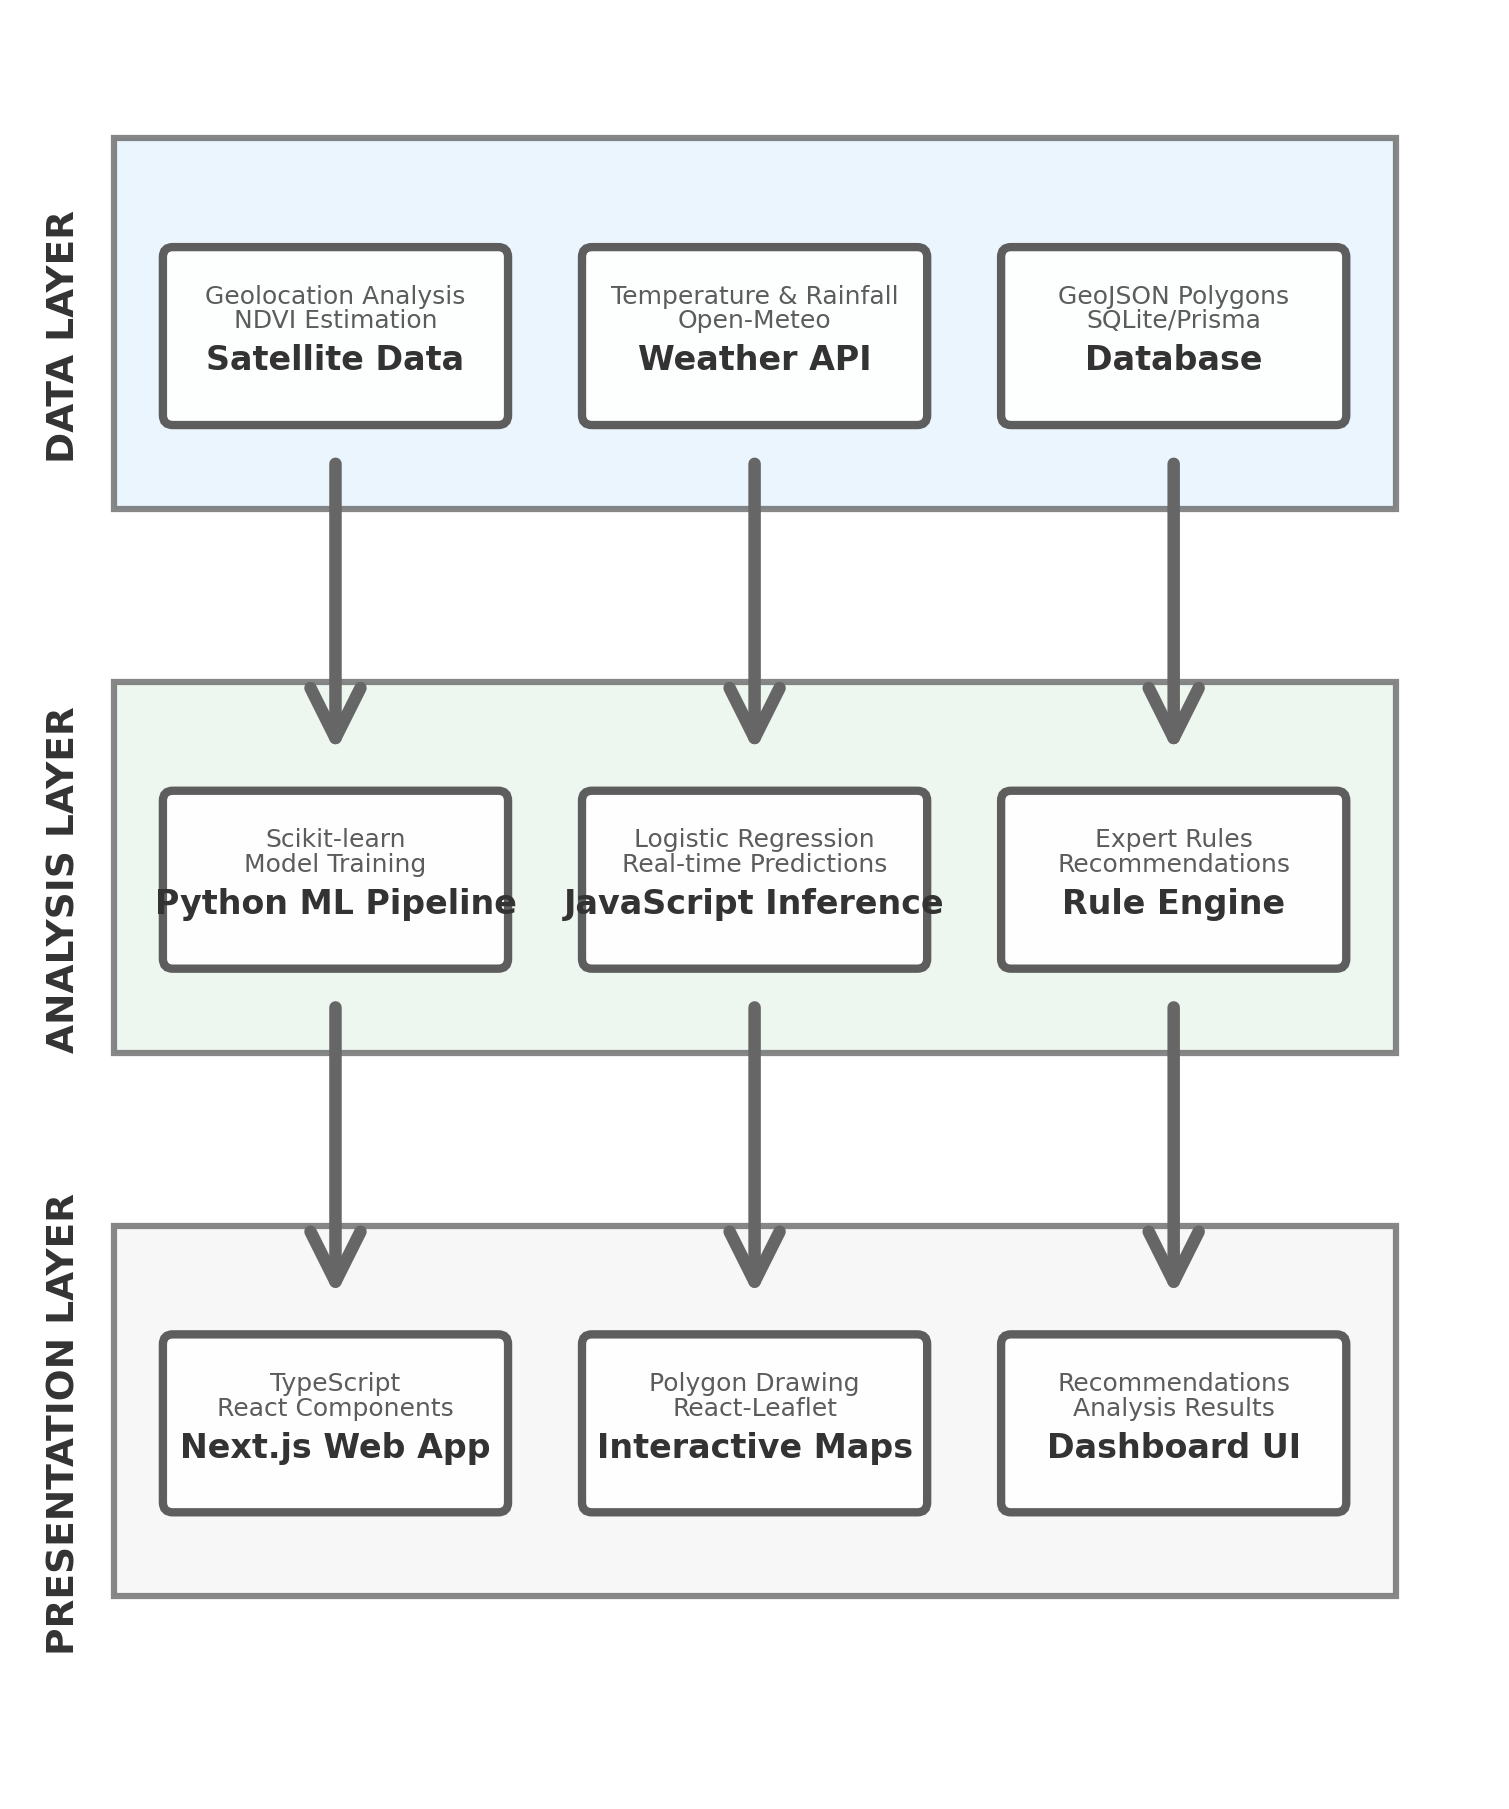
\includegraphics[width=3.5in]{system_architecture_diagram.png}
\caption{System architecture showing the three-layer design: Data Layer (satellite and weather data acquisition), Analysis Layer (ML model training and inference), and Presentation Layer (Next.js web application).}
\label{fig:architecture}
\end{figure}

\subsection{Data Collection and Feature Engineering}

The system collects and processes several types of data for each field analysis:

\textbf{Spatial Data:} Users define field boundaries by drawing polygons on an interactive map. The polygon coordinates are stored as GeoJSON and used to calculate field area and centroid location. The centroid coordinates enable targeted data retrieval for the specific field location.

\textbf{NDVI Data:} For the prototype, NDVI values are estimated based on geolocation and regional vegetation characteristics. The system classifies regions as arid, tropical, or temperate based on latitude and longitude, then generates NDVI estimates consistent with typical values for each region type. In a production system, this would be replaced with actual satellite imagery from Sentinel-2 or Landsat missions via Google Earth Engine or Sentinel Hub APIs.

\textbf{Weather Data:} Historical weather data for the 14 days preceding analysis is retrieved from the Open-Meteo API using the field centroid coordinates. Daily temperature and precipitation values are aggregated to compute average temperature and total rainfall features.

Feature engineering transforms raw data into model inputs:

\begin{itemize}
\item \textbf{mean\_ndvi}: Average NDVI value across the field and time period
\item \textbf{ndvi\_trend}: Temporal slope indicating vegetation change direction
\item \textbf{ndvi\_variance}: Spatial or temporal variance indicating uniformity
\item \textbf{avg\_temperature\_c}: Mean temperature over the observation period
\item \textbf{total\_rainfall\_mm}: Cumulative precipitation over the observation period
\end{itemize}

\subsection{Machine Learning Model}

A logistic regression classifier was selected for crop health classification based on several considerations: interpretability, computational efficiency, and suitability for the three-class classification problem. The model predicts one of three health status categories:

\begin{itemize}
\item \textbf{HEALTHY}: NDVI values above 0.6 with stable or improving trends
\item \textbf{MODERATE\_STRESS}: NDVI values between 0.45 and 0.6 with potential declining trends
\item \textbf{HIGH\_STRESS}: NDVI values below 0.45 indicating significant vegetation stress
\end{itemize}

The training dataset consists of 610 synthetic samples generated based on agronomic knowledge and typical NDVI-weather relationships for tobacco crops. While synthetic data has limitations, it provides a foundation for prototype development and can be replaced with real field observations as they become available.

The model training process follows standard machine learning practices:

\begin{enumerate}
\item Data splitting: 80\% training, 20\% testing with stratified sampling
\item Model training: Logistic regression with L2 regularization (max iterations: 1000)
\item Evaluation: Classification report, confusion matrix, and accuracy metrics
\item Export: Model coefficients saved to JSON format for web application consumption
\end{enumerate}

\subsection{Recommendation System}

The recommendation system employs rule-based logic to translate model predictions and feature values into actionable advice. Four primary recommendation rules are implemented:

\textbf{Rule 1 - Water Stress Detection:}
\begin{verbatim}
IF mean_ndvi < 0.45 AND total_rainfall < 10mm
THEN recommend irrigation
\end{verbatim}

\textbf{Rule 2 - Monitoring Alert:}
\begin{verbatim}
IF ndvi_trend = DECLINING AND 
   0.45 <= mean_ndvi <= 0.6
THEN recommend close monitoring
\end{verbatim}

\textbf{Rule 3 - Stable Crop:}
\begin{verbatim}
IF mean_ndvi > 0.6 AND 
   (ndvi_trend = STABLE OR IMPROVING)
THEN indicate no immediate action needed
\end{verbatim}

\textbf{Rule 4 - Disease Risk:}
\begin{verbatim}
IF ndvi_variance > 0.05 AND 
   avg_temperature > 25°C
THEN recommend field inspection
\end{verbatim}

Each recommendation includes explanatory text that connects the advice to observed data patterns, enhancing transparency and farmer trust.

\section{Implementation}

\subsection{Machine Learning Pipeline}

The machine learning pipeline is implemented in Python using scikit-learn, pandas, and matplotlib. The codebase is organized into modular components:

\textbf{config.py:} Centralizes configuration parameters including file paths, feature column names, and model hyperparameters.

\textbf{train\_health\_model.py:} Implements the training workflow, including data loading, model training, evaluation, and persistence. The script generates a classification report and confusion matrix visualization saved to the reports directory.

\textbf{export\_model.py:} Converts the trained scikit-learn model into a JSON format containing model coefficients, intercepts, and class labels. This enables model inference in JavaScript without requiring a Python runtime.

The training process produces several artifacts:
\begin{itemize}
\item \texttt{crop\_health\_model.joblib}: Serialized scikit-learn model for Python use
\item \texttt{crop\_health\_model.json}: Model weights in JSON format for web application
\item \texttt{thresholds.json}: Rule-based threshold values for recommendation logic
\item \texttt{training\_summary.md}: Evaluation metrics and performance report
\item \texttt{confusion\_matrix.png}: Visualization of model performance
\end{itemize}

\subsection{Web Application}

The web application is built using Next.js 14 with the App Router architecture, TypeScript for type safety, and Prisma for database management. Key implementation components include:

\textbf{Database Schema:} The Prisma schema defines three models: User (authentication), Field (spatial data and metadata), and Analysis (results and recommendations). SQLite is used as the database engine for simplicity in the prototype phase.

\textbf{Authentication:} User authentication is implemented using bcrypt for password hashing and session management through HTTP-only cookies. The authentication system supports signup, login, and logout operations.

\textbf{Map Interface:} Interactive maps are implemented using React-Leaflet, a React wrapper for the Leaflet mapping library. The PolygonDrawer component enables users to draw field boundaries using Leaflet.draw, with polygon coordinates automatically captured and stored as GeoJSON.

\textbf{Analysis API:} The analysis endpoint (\texttt{/api/analyse}) orchestrates the complete analysis workflow:
\begin{enumerate}
\item Retrieve field polygon from database
\item Fetch satellite and weather data using the satellite module
\item Apply feature engineering transformations
\item Load ML model weights and perform inference
\item Apply recommendation rules
\item Store results in Analysis table
\item Return formatted results to client
\end{enumerate}

\textbf{Results Visualization:} The analysis results page presents information in four sections: (1) field summary with overall health status badge, (2) collapsible raw data table showing NDVI and weather values, (3) health classification with confidence indicators, and (4) prioritized recommendations with explanatory text.

\subsection{Deployment Considerations}

The system is designed for straightforward deployment:
\begin{itemize}
\item \textbf{Frontend and API:} Can be deployed to Vercel, Netlify, or similar platforms supporting Next.js
\item \textbf{Database:} SQLite for development; PostgreSQL recommended for production
\item \textbf{External Dependencies:} Only requires Open-Meteo API (free, no authentication)
\item \textbf{Model Updates:} New model versions can be deployed by replacing JSON files without code changes
\end{itemize}

\section{Results and Evaluation}

\subsection{Model Performance}

The logistic regression classifier achieved strong performance on the test set (122 samples):

\begin{itemize}
\item \textbf{Overall Accuracy:} 97\%
\item \textbf{HEALTHY class:} Precision 0.97, Recall 1.00, F1-score 0.99
\item \textbf{HIGH\_STRESS class:} Precision 1.00, Recall 0.94, F1-score 0.97
\item \textbf{MODERATE\_STRESS class:} Precision 0.93, Recall 0.97, F1-score 0.95
\end{itemize}

The confusion matrix (Fig. \ref{fig:confusion}) reveals minimal misclassification, with most errors occurring between adjacent stress categories (MODERATE\_STRESS and HIGH\_STRESS), which is acceptable given the continuous nature of crop health.

\begin{figure}[!t]
\centering
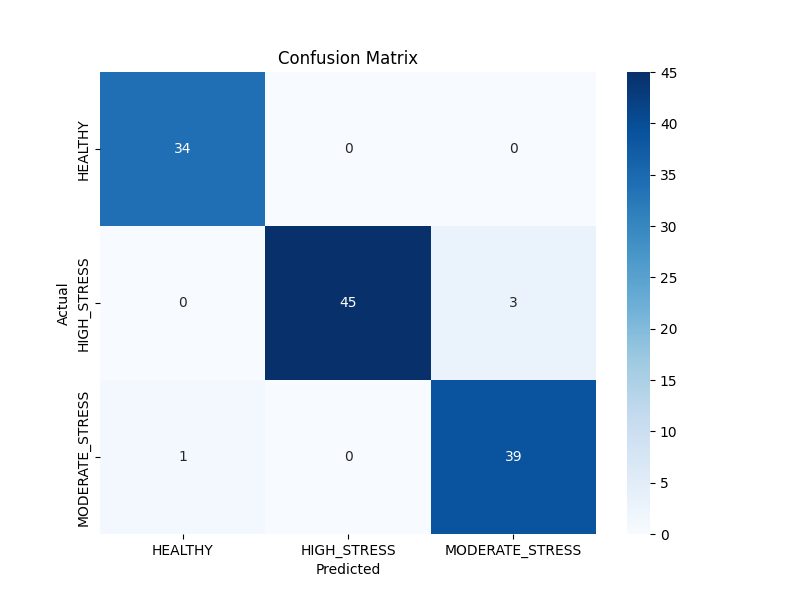
\includegraphics[width=3.5in]{model_confusion_matrix.png}
\caption{Confusion matrix showing classification performance across three health categories. The model achieves 97\% overall accuracy with minimal misclassification between adjacent stress levels.}
\label{fig:confusion}
\end{figure}

The high performance metrics validate the feature engineering approach and demonstrate that NDVI combined with weather data provides sufficient information for crop health classification. The model's simplicity (logistic regression) ensures interpretability, allowing agronomists to understand and validate the decision boundaries.

\subsection{System Functionality}

The prototype successfully implements all planned features:

\textbf{User Management:} Registration and authentication work reliably, with passwords securely hashed and sessions properly managed.

\textbf{Field Definition:} The polygon drawing interface enables intuitive field boundary definition. Polygon coordinates are correctly captured and stored, with automatic area calculation.

\textbf{Data Integration:} Weather data retrieval from Open-Meteo API functions consistently, providing accurate historical meteorological information for field locations.

\textbf{Analysis Execution:} The complete analysis pipeline executes in under 3 seconds for typical field sizes, providing responsive user experience.

\textbf{Results Presentation:} Analysis results are clearly presented with appropriate visualizations and explanatory text. Recommendations are specific and actionable.

\subsection{Limitations and Validation}

Several limitations should be acknowledged:

\textbf{NDVI Estimation:} The current prototype uses geolocation-based NDVI estimation rather than actual satellite imagery. While this demonstrates the system architecture, production deployment requires integration with real satellite data sources such as Sentinel Hub or Google Earth Engine.

\textbf{Training Data:} The model is trained on synthetic data generated based on agronomic knowledge rather than real field observations. Validation with actual tobacco field data is necessary to confirm model accuracy in operational conditions.

\textbf{Temporal Resolution:} The system currently performs point-in-time analysis rather than continuous monitoring. Implementing time-series analysis would enable trend detection and seasonal pattern recognition.

\textbf{Crop Specificity:} While designed for tobacco, the system has not been validated for other crop types. Feature importance and threshold values may differ for other agricultural products.

\textbf{Spatial Resolution:} The system treats each field as a homogeneous unit, computing single aggregate values. Within-field variability analysis would require higher resolution data and more sophisticated spatial processing.

\section{Discussion}

This research demonstrates the feasibility of developing accessible, web-based crop monitoring systems using freely available satellite and weather data. The prototype successfully addresses several key challenges in agricultural technology adoption:

\textbf{Accessibility:} By using open data sources and web technologies, the system eliminates cost barriers that prevent smallholder farmers from accessing precision agriculture tools. The web-based interface requires no specialized software installation.

\textbf{Explainability:} The combination of a simple machine learning model with rule-based recommendations ensures that system outputs can be understood and validated by agronomists and farmers. Each recommendation is accompanied by explanatory text linking advice to observed data patterns.

\textbf{Scalability:} The architecture separates model training (Python) from inference (JavaScript), enabling the web application to serve many users without requiring Python runtime infrastructure. Model updates can be deployed independently of application code.

\textbf{Extensibility:} The modular design facilitates future enhancements such as integration with real satellite APIs, incorporation of additional data sources (soil data, pest reports), and expansion to other crop types.

The high model accuracy (97\%) suggests that the selected features effectively capture crop health status. However, validation with real field data remains essential. The next phase of research should focus on collecting ground truth data from actual tobacco fields, including farmer observations, yield measurements, and expert assessments.

The recommendation system's rule-based approach provides transparency but may lack the sophistication needed for complex scenarios. Future work could explore hybrid approaches combining machine learning predictions with expert system rules, or reinforcement learning methods that optimize recommendations based on outcome feedback.

Integration with actual satellite imagery services represents the most critical enhancement for production deployment. Google Earth Engine provides free access to Sentinel-2 and Landsat imagery with global coverage and regular updates. Implementing this integration would enable true operational monitoring with 5-10 day revisit frequencies.

\section{Conclusion}

This paper presented a web-based prototype system for tobacco crop health monitoring using satellite data and machine learning. The system successfully demonstrates how freely available remote sensing data can be combined with simple machine learning models to provide actionable agricultural insights.

Key contributions include: (1) a complete system architecture separating model training from web-based inference, (2) a logistic regression classifier achieving 97\% accuracy in crop health classification, (3) an explainable recommendation system translating technical data into farming advice, and (4) a user-friendly web interface enabling farmers to define fields and access analysis results.

The prototype validates the technical feasibility of the approach while identifying clear paths for enhancement. Integration with real satellite imagery services, validation with field data, and expansion of the recommendation system represent priority areas for future development.

As satellite data becomes increasingly accessible and machine learning tools more sophisticated, systems like this have the potential to democratize precision agriculture, enabling smallholder farmers to make data-driven decisions that improve productivity and sustainability.

\section*{Acknowledgment}

The authors would like to thank the open-source community for providing the tools and libraries that made this research possible, including Next.js, React-Leaflet, scikit-learn, and the Open-Meteo project.

\begin{thebibliography}{00}

\bibitem{rouse1974monitoring} J. W. Rouse, R. H. Haas, J. A. Schell, and D. W. Deering, ``Monitoring vegetation systems in the Great Plains with ERTS,'' in \textit{Third Earth Resources Technology Satellite-1 Symposium}, vol. 1, 1974, pp. 309--317.

\bibitem{tucker1979red} C. J. Tucker, ``Red and photographic infrared linear combinations for monitoring vegetation,'' \textit{Remote Sensing of Environment}, vol. 8, no. 2, pp. 127--150, 1979.

\bibitem{weiss2020remote} M. Weiss, F. Jacob, and G. Duveiller, ``Remote sensing for agricultural applications: A meta-review,'' \textit{Remote Sensing of Environment}, vol. 236, p. 111402, 2020.

\bibitem{gorelick2017google} N. Gorelick, M. Hancher, M. Dixon, S. Ilyushchenko, D. Thau, and R. Moore, ``Google Earth Engine: Planetary-scale geospatial analysis for everyone,'' \textit{Remote Sensing of Environment}, vol. 202, pp. 18--27, 2017.

\bibitem{liakos2018machine} K. G. Liakos, P. Busato, D. Moshou, S. Pearson, and D. Bochtis, ``Machine learning in agriculture: A review,'' \textit{Sensors}, vol. 18, no. 8, p. 2674, 2018.

\bibitem{chlingaryan2018machine} A. Chlingaryan, S. Sukkarieh, and B. Whelan, ``Machine learning approaches for crop yield prediction and nitrogen status estimation in precision agriculture: A review,'' \textit{Computers and Electronics in Agriculture}, vol. 151, pp. 61--69, 2018.

\bibitem{kamilaris2018deep} A. Kamilaris and F. X. Prenafeta-Boldú, ``Deep learning in agriculture: A survey,'' \textit{Computers and Electronics in Agriculture}, vol. 147, pp. 70--90, 2018.

\bibitem{rose2016decision} D. C. Rose, W. J. Sutherland, C. Parker, M. Lobley, M. Winter, C. Morris, S. Twining, C. Ffoulkes, T. Amano, and L. V. Dicks, ``Decision support tools for agriculture: Towards effective design and delivery,'' \textit{Agricultural Systems}, vol. 149, pp. 165--174, 2016.

\bibitem{wolfert2017big} S. Wolfert, L. Ge, C. Verdouw, and M. J. Bogaardt, ``Big data in smart farming--a review,'' \textit{Agricultural Systems}, vol. 153, pp. 69--80, 2017.

\end{thebibliography}

\vspace{12pt}

\end{document}
